\section{等价改写}
\label{sec:cone-rewrite}

实际问题很少一开始就长成式~\eqref{eq:cone-qp}或式~\eqref{eq:cone-conic}的样子，常要引入辅助变量才能写进去。这就需要回答：引入辅助变量、换了约束之后，凭什么说问题没有变？

\paragraph{什么叫没有改变问题}
设原问题是在$\bm{C}$上最小化$f(\bm{x})$，改写后的问题是在$\bm{C}'$上最小化$\phi(\bm{x},\bm{z})$，其中$\bm{z}$是辅助变量。要说二者等价，需要两个方向的对应。

\begin{definition}[等价改写]
\label{def:cone-equivalent}
若下面两条都成立，则称改写后的问题是原问题的\term{等价改写}（equivalent reformulation）：
\begin{enumerate}
 \item 对每个$\bm{x}\in\bm{C}$，存在$\bm{z}$使$(\bm{x},\bm{z})\in\bm{C}'$，且$\phi(\bm{x},\bm{z})\leq f(\bm{x})$；
 \item 对每个$(\bm{x},\bm{z})\in\bm{C}'$，都有$\bm{x}\in\bm{C}$，且$f(\bm{x})\leq\phi(\bm{x},\bm{z})$。
\end{enumerate}
\end{definition}

第一条说原问题的每个候选都有替身，而且替身的代价不更高。第二条说消去辅助变量后回到的正是原约束，代价也没有被低估。

\begin{theorem}[等价改写保持最优值与最优解]
\label{thm:cone-equivalent}
在定义~\ref{def:cone-equivalent}的条件下，两个问题的最优值相等。若$(\bm{x}^\star,\bm{z}^\star)$是改写问题的最优解，则$\bm{x}^\star$是原问题的最优解。若$\bm{x}^\star$是原问题的最优解，则它配上第一条中的$\bm{z}$是改写问题的最优解。
\end{theorem}

\begin{proof}
记两个最优值为$p$和$p'$。第一条说明，原问题的每个目标值都不低于改写问题的某个目标值，于是$p'\leq p$。第二条同理给出$p\leq p'$，所以$p=p'$。

设$(\bm{x}^\star,\bm{z}^\star)$最优。第二条给出$\bm{x}^\star\in\bm{C}$，以及
\[
 f(\bm{x}^\star)\leq\phi(\bm{x}^\star,\bm{z}^\star)=p'=p.
\]
所以$\bm{x}^\star$最优。

设$\bm{x}^\star$最优，取第一条中的$\bm{z}$。则$(\bm{x}^\star,\bm{z})$可行，且
\[
 \phi(\bm{x}^\star,\bm{z})\leq f(\bm{x}^\star)=p=p'.
\]
所以它最优。
\end{proof}

定理同时给出了恢复原变量的办法：解改写问题，然后把辅助变量丢掉。对照图~\ref{fig:cone-rewrite-project}(a)，改写后的可行集沿辅助变量方向投影，恰好覆盖原可行集。

\begin{BookInlineFigure}
  \centering
  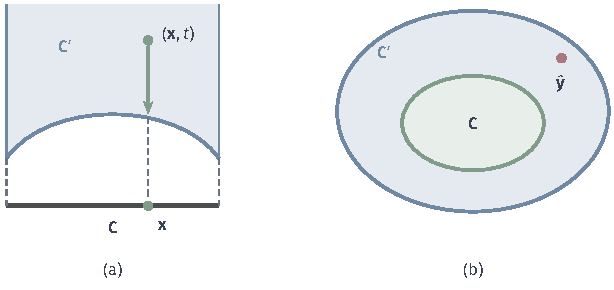
\includegraphics[width=104mm]{figures/05-optimization/06-constrained-optimization/tikz/cone-rewrite-project/figure.pdf}
  \caption{等价改写与松弛的区别。(a)等价改写：点$(\bm{x},t)$沿竖直方向下移不增加代价，投影后回到$\bm{C}$，$\bm{C}'$的投影恰是$\bm{C}$（深灰线段）。(b)松弛：$\bm{C}'$严格包含$\bm{C}$，$\bm{C}'$中可能有红点$\hat{\bm{y}}$这样不对应任何原可行点的元素，所以只保留定义中的第一条。}
  \label{fig:cone-rewrite-project}
\end{BookInlineFigure}

若只有第一条成立，得到的是另一种东西：改写后的问题最优值不超过原问题，但它的解可能不对应任何原可行点。这就是图中的(b)，留到第~\ref{sec:cone-relax}节讨论。

\subsection{上图形式}
\label{sec:cone-epigraph}

目标是非线性函数时，能否把非线性移到约束里，使目标变成线性的？这一小节用范数和凸二次两种目标回答这个问题。

\paragraph{范数目标}
函数$f$的\term{上图}（epigraph）是它图像上方的点集$\{(\bm{x},t):f(\bm{x})\leq t\}$。最小化$f$，就是在上图中寻找最低的点。

对$\min\lVert\bm{D}\bm{x}-\bm{r}\rVert_2$，引入$t$，写成
\begin{equation}
 \min_{\bm{x},t}\ t\quad\text{s.t.}\quad\lVert\bm{D}\bm{x}-\bm{r}\rVert_2\leq t.
 \label{eq:cone-norm-epigraph}
\end{equation}
目标成了线性函数，约束是一条二阶锥约束。

核对定义~\ref{def:cone-equivalent}。对任意$\bm{x}$，取$t=\lVert\bm{D}\bm{x}-\bm{r}\rVert_2$，可行，代价相等，第一条成立。对任意可行的$(\bm{x},t)$，$\lVert\bm{D}\bm{x}-\bm{r}\rVert_2\leq t$，第二条成立。

最优时约束取等号：若$t>\lVert\bm{D}\bm{x}-\bm{r}\rVert_2$，把$t$减小到等号处仍可行，目标更低。图~\ref{fig:cone-epigraph}(a)中的绿色箭头就是这个下移。

\begin{BookInlineFigure}
  \centering
  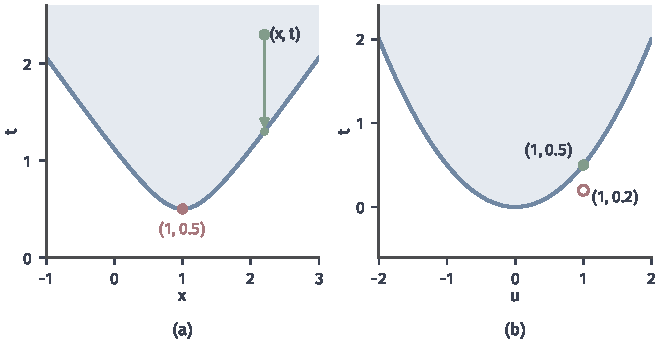
\includegraphics[width=112mm]{figures/05-optimization/06-constrained-optimization/matplotlib/cone-epigraph/figure.pdf}
  \caption{上图改写。(a)$f(x)=\lVert(x-1,1/2)\rVert_2$的上图（浅蓝），绿点下移到函数图像上时$t$减小而$x$不变，红点是上图中的最低点。(b)在网格上逐点判定$\lVert(2u,2t-1)\rVert_2\leq2t+1$，浅蓝区域恰是抛物线$t\geq u^2/2$的上方，绿点$(1,0.5)$在边界上，红色空心点$(1,0.2)$不满足约束。}
  \label{fig:cone-epigraph}
\end{BookInlineFigure}

\paragraph{凸二次目标}
平方范数多了一层：$\frac12\bm{x}^\top\bm{Q}\bm{x}\leq t$的左端是二次的，不是范数。这需要两步转换。

第一步是分解。$\bm{Q}\succeq\bm{0}$时存在$\bm{F}\in\mathbb{R}^{k\times n}$使$\bm{Q}=\bm{F}^\top\bm{F}$，例如取Cholesky因子或由谱分解得到。最小二乘中直接有$\bm{F}=\bm{D}$。于是上图约束是$\lVert\bm{F}\bm{x}\rVert_2^2\leq2t$。

第二步把“平方范数不超过乘积”写成二阶锥。

\begin{lemma}[旋转二阶锥]
\label{lem:cone-rotated-soc}
对$\bm{u}\in\mathbb{R}^k$和$s,w\in\mathbb{R}$，
\begin{equation}
 \lVert\bm{u}\rVert_2^2\leq sw,\quad s\geq0,\quad w\geq0
 \quad\Longleftrightarrow\quad
 \left\lVert\begin{bmatrix}2\bm{u}\\s-w\end{bmatrix}\right\rVert_2\leq s+w.
 \label{eq:cone-rotated-soc}
\end{equation}
\end{lemma}

\begin{proof}
先证从左到右。由$\lVert\bm{u}\rVert_2^2\leq sw$，
\[
 4\lVert\bm{u}\rVert_2^2+(s-w)^2\leq4sw+(s-w)^2=(s+w)^2.
\]
又$s+w\geq0$，两边开方得到右式。

再证从右到左。右式的范数不小于$\lvert s-w\rvert$，所以$s+w\geq\lvert s-w\rvert$。分别取绝对值的两种符号，得到$w\geq0$和$s\geq0$。把右式平方，同样的展开给出$4\lVert\bm{u}\rVert_2^2\leq4sw$。
\end{proof}

取$\bm{u}=\bm{F}\bm{x}$、$s=2t$、$w=1$，就得到$\lVert\bm{F}\bm{x}\rVert_2^2\leq2t$的二阶锥形式。凸二次规划~\eqref{eq:cone-qp}因而等价于
\begin{equation}
 \begin{aligned}
 \min_{\bm{x},t}\quad&t+\bm{q}^\top\bm{x}\\
 \text{s.t.}\quad&\left\lVert\begin{bmatrix}2\bm{F}\bm{x}\\2t-1\end{bmatrix}\right\rVert_2\leq2t+1,\\
 &\bm{A}\bm{x}=\bm{b},\quad\bm{G}\bm{x}\leq\bm{h}.
 \end{aligned}
 \label{eq:cone-qp-socp}
\end{equation}
图~\ref{fig:cone-epigraph}(b)用网格判定的方式核对了$k=1$的情形：约束$\lVert(2u,2t-1)\rVert_2\leq2t+1$的解集正好是$t\geq u^2/2$。

再用定义~\ref{def:cone-equivalent}核对。第一条取$t=\frac12\bm{x}^\top\bm{Q}\bm{x}$。第二条由引理得到$t\geq\frac12\bm{x}^\top\bm{Q}\bm{x}$，于是原目标不超过改写后的目标。恢复$\bm{x}$时丢弃$t$即可。

\begin{example}[预算问题的二阶锥形式]
\label{ex:cone-budget-socp}
预算问题的目标是$\frac12\lVert\bm{D}\bm{x}-\bm{r}\rVert_2^2$，这里取$\bm{u}=\bm{D}\bm{x}-\bm{r}$，约束写成
\[
 \left\lVert\begin{bmatrix}2(\bm{D}\bm{x}-\bm{r})\\2t-1\end{bmatrix}\right\rVert_2\leq2t+1.
\]
在$\bm{x}^\star=(3/2,1/2)$处，残差是$(-2,1/2,1/2)$，取$t=9/4$。左端向量是$(-4,1,1,7/2)$，长度的平方是
\[
 16+1+1+\frac{49}{4}=\frac{121}{4}.
\]
所以左端等于$11/2$，右端也等于$2t+1=11/2$。约束取等号，改写问题的目标值$t=9/4$与原问题的$f^\star$相同。
\end{example}

只有$\bm{Q}\succeq\bm{0}$时才有实分解$\bm{Q}=\bm{F}^\top\bm{F}$。第~\ref{sec:cone-nonconvex-qp}小节的$\operatorname{diag}(1,-1)$没有这样的分解，也不可能写成式~\eqref{eq:cone-qp-socp}：二阶锥规划的可行集是凸的，而目标的上图不凸。

另外，若目标是$\min\lVert\bm{D}\bm{x}-\bm{r}\rVert_2^2$，也可以直接最小化不带平方的范数。平方在非负数上严格递增，所以两者最优解相同；但最优值不同，这与定义~\ref{def:cone-equivalent}的“最优值相等”不是一回事，恢复目标值时要重新平方。

\paragraph{维数与成本}
增加变量并不自动带来计算上的好处。表~\ref{tab:cone-epi-cost}比较凸二次目标的两种写法，$\bm{Q}=\bm{F}^\top\bm{F}$，$\bm{F}\in\mathbb{R}^{k\times n}$。

\begin{BookInlineTable}
  \centering
  \begin{tabular}{lll}
    \toprule
    & 二次规划形式 & 二阶锥形式\\
    \midrule
    变量个数 & $n$ & $n+1$\\
    非线性结构 & 目标中的$\bm{Q}$ & 一个$k+2$维的二阶锥\\
    需要的准备 & $\bm{Q}$或矩阵向量积 & 分解$\bm{F}$\\
    可用的方法 & 二次规划专用方法 & 通用锥规划方法\\
    \bottomrule
  \end{tabular}
  \caption{同一凸二次目标的两种写法。}
  \label{tab:cone-epi-cost}
\end{BookInlineTable}

$\bm{Q}$稀疏时，分解因子$\bm{F}$可能比$\bm{Q}$稠密得多，改写后存储反而增加。$\bm{Q}$只能通过矩阵向量积访问时，分解根本做不出来。反过来，$\bm{Q}=\bm{D}^\top\bm{D}$稠密而$\bm{D}$稀疏时，直接用$\bm{F}=\bm{D}$比存$\bm{Q}$便宜。

改写的价值在于让问题能交给统一的求解方法，能和其他范数约束混用。只有二次目标和线性约束时，保留原形式通常更省。

\subsection{Schur补改写}
\label{sec:cone-schur}

二次上界和矩阵的逆都不是矩阵元素的线性函数。这一小节回答：这种限制能否写成线性矩阵不等式？工具是Schur补，关键是分清哪一块必须正定。

\paragraph{从配方到判据}
先看$2\times2$的情形。设$p>0$，考虑二次型
\[
 pa^2+2nab+Tb^2.
\]
配方得到
\[
 p\Bigl(a+\frac{n}{p}b\Bigr)^2+\Bigl(T-\frac{n^2}{p}\Bigr)b^2.
\]
第一项可以用$a$消成零，所以整个二次型非负，取决于第二项的系数$T-n^2/p$是否非负。

矩阵版本完全类似，只是把除以$p$换成乘以逆矩阵。

\begin{lemma}[Schur补判据]
\label{lem:cone-schur}
设对称矩阵分块为
\begin{equation}
 \bm{M}=\begin{bmatrix}\bm{P}&\bm{N}\\\bm{N}^\top&\bm{T}\end{bmatrix},
 \label{eq:cone-block-matrix}
\end{equation}
其中$\bm{P}\succ\bm{0}$。则
\begin{equation}
 \bm{M}\succeq\bm{0}\quad\Longleftrightarrow\quad\bm{T}-\bm{N}^\top\bm{P}^{-1}\bm{N}\succeq\bm{0}.
 \label{eq:cone-schur}
\end{equation}
矩阵$\bm{T}-\bm{N}^\top\bm{P}^{-1}\bm{N}$称为$\bm{P}$在$\bm{M}$中的\term{Schur补}（Schur complement）。
\end{lemma}

\begin{proof}
对任意向量$\bm{a},\bm{b}$，记$\bm{S}=\bm{T}-\bm{N}^\top\bm{P}^{-1}\bm{N}$。配方得到
\[
 \begin{bmatrix}\bm{a}\\\bm{b}\end{bmatrix}^\top\bm{M}\begin{bmatrix}\bm{a}\\\bm{b}\end{bmatrix}
 =(\bm{a}+\bm{P}^{-1}\bm{N}\bm{b})^\top\bm{P}(\bm{a}+\bm{P}^{-1}\bm{N}\bm{b})+\bm{b}^\top\bm{S}\bm{b}.
\]
若$\bm{S}\succeq\bm{0}$，右端两项都非负，$\bm{M}\succeq\bm{0}$。

反过来，设$\bm{M}\succeq\bm{0}$。对任意$\bm{b}$，取$\bm{a}=-\bm{P}^{-1}\bm{N}\bm{b}$，第一项变为零，于是$\bm{b}^\top\bm{S}\bm{b}\geq0$。
\end{proof}

式~\eqref{eq:cone-schur}的左端对$\bm{P},\bm{N},\bm{T}$是线性的，右端含有逆和乘积。这就是改写的用处：把弯曲的右端换成线性的左端。

\paragraph{二次型上界}
令$\bm{P}=\bm{I}$、$\bm{N}=\bm{u}$、$\bm{T}=t$，由引理~\ref{lem:cone-schur}，
\begin{equation}
 \lVert\bm{u}\rVert_2^2\leq t\quad\Longleftrightarrow\quad\begin{bmatrix}\bm{I}&\bm{u}\\\bm{u}^\top&t\end{bmatrix}\succeq\bm{0}.
 \label{eq:cone-schur-quadratic}
\end{equation}
代入$\bm{u}=\bm{D}\bm{x}-\bm{r}$，左端对$\bm{x}$是二次的，右端的矩阵对$(\bm{x},t)$却是仿射的。这条约束就是一条线性矩阵不等式，和式~\eqref{eq:cone-lmi}同型。这里单位块$\bm{I}$恒正定，引理的条件自动满足。

以预算问题的解为例，$\lVert\bm{u}\rVert_2^2=9/2$。取$t=9/2$，矩阵是$4\times4$的，它的Schur补为零，矩阵半正定且奇异。取$t$更小，Schur补为负，矩阵不再半正定。

\paragraph{含逆矩阵的限制}
再看一个$\bm{P}$本身是变量的例子。设$\bm{Y}\succ\bm{0}$是对称矩阵变量，$\bm{b}$是向量，由引理~\ref{lem:cone-schur}，
\begin{equation}
 \bm{b}^\top\bm{Y}^{-1}\bm{b}\leq t\quad\Longleftrightarrow\quad\begin{bmatrix}\bm{Y}&\bm{b}\\\bm{b}^\top&t\end{bmatrix}\succeq\bm{0}\qquad(\bm{Y}\succ\bm{0}).
 \label{eq:cone-schur-inverse}
\end{equation}
右端是$(\bm{Y},\bm{b},t)$的线性矩阵不等式，也说明左端的函数在$\bm{Y}\succ\bm{0}$上对$(\bm{Y},\bm{b})$联合凸：它的上图由一条线性矩阵不等式定义。

用数值走一遍。取
\[
 \bm{Y}=\begin{bmatrix}2&1\\1&2\end{bmatrix},\qquad\bm{b}=\begin{bmatrix}1\\1\end{bmatrix}.
\]
矩阵的逆是
\[
 \bm{Y}^{-1}=\frac13\begin{bmatrix}2&-1\\-1&2\end{bmatrix}.
\]
代入得到
\[
 \bm{b}^\top\bm{Y}^{-1}\bm{b}=\frac13(2-1-1+2)=\frac23.
\]
$3\times3$块矩阵的行列式等于$\det\bm{Y}$与Schur补的乘积，
\[
 \det\bm{M}=3\Bigl(t-\frac23\Bigr).
\]
于是$t<2/3$时矩阵不半正定，$t=2/3$时恰好在边界上。数值上，$t=1/2$时最小特征值约为$-0.137$，$t=1$时约为$0.268$。图~\ref{fig:cone-schur}(a)画出最小特征值穿过零点的过程。

\begin{BookInlineFigure}
  \centering
  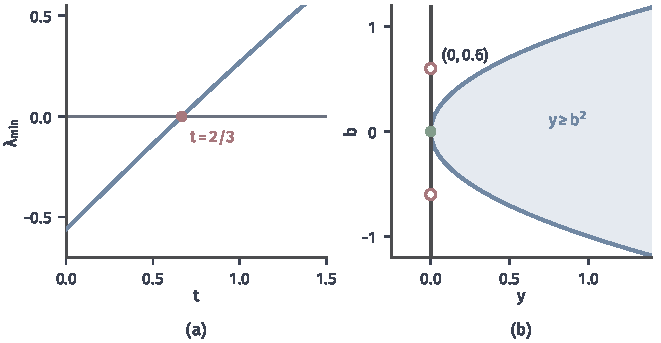
\includegraphics[width=112mm]{figures/05-optimization/06-constrained-optimization/matplotlib/cone-schur/figure.pdf}
  \caption{Schur补判据及其边界。(a)式~\eqref{eq:cone-schur-inverse}的块矩阵的最小特征值随$t$的变化，红点是$t=2/3$。(b)$\begin{bmatrix}y&b\\b&1\end{bmatrix}\succeq\bm{0}$的解集（浅蓝）是抛物线$y\geq b^2$的内部及边界。深灰线$y=0$上只有绿点$(0,0)$可行，红色空心点$(0,\pm0.6)$不可行。}
  \label{fig:cone-schur}
\end{BookInlineFigure}

\paragraph{奇异的情形}
$\bm{P}$只半正定时，不能写$\bm{P}^{-1}$，把逆换成伪逆也不够。看一个例子：
\[
 \begin{bmatrix}0&1\\1&1\end{bmatrix}.
\]
这里$\bm{P}=0$，伪逆也是$0$，“Schur补”算出来是$1\geq0$。但矩阵的行列式是$-1$，它不半正定。缺的是一个像空间的条件：$\bm{P}$的零方向上，$\bm{N}$也必须为零。

\begin{lemma}[奇异情形的Schur补判据]
\label{lem:cone-schur-singular}
在引理~\ref{lem:cone-schur}的分块中，设$\bm{P}\succeq\bm{0}$，$\bm{P}^\dagger$是其伪逆。则$\bm{M}\succeq\bm{0}$，当且仅当
\begin{equation}
 (\bm{I}-\bm{P}\bm{P}^\dagger)\bm{N}=\bm{0}\quad\text{且}\quad\bm{T}-\bm{N}^\top\bm{P}^\dagger\bm{N}\succeq\bm{0}.
 \label{eq:cone-schur-singular}
\end{equation}
\end{lemma}

\begin{proof}
设$\bm{M}\succeq\bm{0}$。任取$\bm{w}\in\ker\bm{P}$和向量$\bm{v}$，把$\bm{M}$的二次型作用在$(\bm{w},\varepsilon\bm{v})$上，得到
\[
 2\varepsilon\bm{w}^\top\bm{N}\bm{v}+\varepsilon^2\bm{v}^\top\bm{T}\bm{v}\geq0.
\]
这对正负的小$\varepsilon$都成立，必有$\bm{w}^\top\bm{N}\bm{v}=0$。所以$\bm{N}$的列与$\ker\bm{P}$正交，属于$\operatorname{range}\bm{P}$，这正是$\bm{P}\bm{P}^\dagger\bm{N}=\bm{N}$。

在条件$\bm{P}\bm{P}^\dagger\bm{N}=\bm{N}$之下，令
\[
 \bm{U}=\begin{bmatrix}\bm{I}&-\bm{P}^\dagger\bm{N}\\\bm{0}&\bm{I}\end{bmatrix},
\]
它可逆。直接相乘，并用$\bm{P}^\dagger\bm{P}\bm{P}^\dagger=\bm{P}^\dagger$，得到
\[
 \bm{U}^\top\bm{M}\bm{U}=\begin{bmatrix}\bm{P}&\bm{0}\\\bm{0}&\bm{T}-\bm{N}^\top\bm{P}^\dagger\bm{N}\end{bmatrix}.
\]
可逆合同变换保持半正定性，所以$\bm{M}\succeq\bm{0}$当且仅当右端半正定，也就是第二个条件成立。这同时完成了两个方向的证明。
\end{proof}

图~\ref{fig:cone-schur}(b)展示了这个条件的几何含义。$\begin{bmatrix}y&b\\b&1\end{bmatrix}\succeq\bm{0}$在$y>0$时等价于$b^2/y\leq1$，即$y\geq b^2$。到$y=0$时，$b^2/y$没有定义，判据要求$b=0$，图中只有原点留下。

这里还有一个定义域的问题。式~\eqref{eq:cone-schur-inverse}要求$\bm{Y}\succ\bm{0}$，而块矩阵半正定只推出$\bm{Y}\succeq\bm{0}$。改写时若丢掉严格正定的要求，集合就多了边界上的奇异$\bm{Y}$，这些点在原问题中$\bm{Y}^{-1}$并无定义。这时要么说明原函数在边界上取什么值，要么在求解后核对$\bm{Y}$是否真的正定。

\paragraph{二阶锥也是线性矩阵不等式}
同样的工具给出
\begin{equation}
 \lVert\bm{u}\rVert_2\leq t\quad\Longleftrightarrow\quad\begin{bmatrix}t\bm{I}&\bm{u}\\\bm{u}^\top&t\end{bmatrix}\succeq\bm{0}.
 \label{eq:cone-soc-as-lmi}
\end{equation}
$t>0$时由引理~\ref{lem:cone-schur}，Schur补是$t-\bm{u}^\top\bm{u}/t$。$t=0$时左上块为零，由引理~\ref{lem:cone-schur-singular}迫使$\bm{u}=\bm{0}$。$t<0$时对角元为负，矩阵不半正定。三种情形都与左式一致。

所以二阶锥规划可以写成半正定规划。这种包含关系的计算含义留到第~\ref{sec:cone-methods}节讨论。
